\documentclass[11.5pt,two column]{llncs}
\usepackage{times}
\usepackage{helvet}
\usepackage{courier}
\usepackage{enumitem}
\usepackage{graphicx}
\usepackage{amssymb, amsmath}
\setcounter{tocdepth}{3}
\usepackage{multicol}
\usepackage{url}
%\usepackage[margin=2pt]{subfig}
\usepackage{xcolor}
\usepackage{tikz}
\usepackage{algorithm}
\usepackage{algpseudocode}
\usepackage{authblk}
\usetikzlibrary{arrows}
\usepackage{enumitem}
\usepackage{sectsty}
\usepackage{array,url}
\usepackage{tikz}
\usetikzlibrary{arrows}
% change the appearance of the tikz arrow for the argumentation networks
% and some other settings to make all the graphs look similar
\tikzset{>=latex,every node/.style={circle, minimum size=0.5cm, draw=black}} 


\addtolength{\oddsidemargin}{-0.85in}
\addtolength{\evensidemargin}{-0.85in}
\addtolength{\textwidth}{1.7in}
\addtolength{\topmargin}{-.7in}
\addtolength{\textheight}{1.3in}
\setlength{\columnsep}{0.3in}

\newcommand{\todo}[1]{{\color{red}\textbf{[TODO: } #1 \textbf{]}}}
\newcommand{\Mark}[1]{\textsuperscript{#1}}
\newcommand{\floris}[1]{{\color{red}\textbf{Floris: }#1}} 

\renewcommand\Authfont{\fontsize{10}{14.4}\selectfont}
\renewcommand\Affilfont{\fontsize{9}{10.8}\selectfont}

\sectionfont{\fontsize{12}{15}\selectfont}
\subsectionfont{\fontsize{10}{15}\selectfont}

\title{RationalGRL: A Framework for Argumentation and Goal Modeling}
\author{Marc van Zee\\
\vspace{-0.35cm}
Computer Science and Communication (CSC), University of Luxembourg\\
2, Avenue de l'Universite, L-4365 Esch-sur-Alzette, Luxembourg\\ marcvanzee@gmail.com
\and
\vspace{-0.4cm}
Diana Marosin\\
\vspace{-0.35cm}
Luxembourg Institute of Science and Technology (LIST)\\
5 Avenue des Hauts-Fourneaux, 4362 Esch-sur-Alzette, Luxembourg\\ diana.marosin@list.lu
\and 
\vspace{-0.4cm}
Floris Bex\\
\vspace{-0.35cm}
Department of Information and Computing Science, Utrecht University\\
Princetonplein 5, 3584 CC Utrecht, Netherlands\\
florisbex@gmail.com
\and
\vspace{-0.4cm}
Sepideh Ghanavati\\
\vspace{-0.35cm}
Department of Computer Science, Texas Tech University\\
2500 Broadway, Lubbock, TX 79409, United States\\
sepideh.ghanavati@ttu.edu
}
\date{}

\begin{document}
\twocolumn[{%
 \centering
 \LARGE RationalGRL: A Framework for Argumentation and Goal Modeling \\[1.5em]
 \large Marc van Zee\Mark{1},
        Diana Marosin\Mark{2},
        Floris Bex\Mark{3},
        and Sepideh Ghanavati\Mark{4}\\[1em]
 \normalsize
 \begin{tabular}{*{4}{>{\centering}p{.22\textwidth}}}
  \Mark{1}Computer Science and Communication (CSC) & \Mark{2}Luxembourg Institute of Science and Technology & \Mark{3}Information and Computing Science & \Mark{4}Department of Computer Science \tabularnewline
  University of Luxembourg & Luxembourg & Utrecht University & Texas Tech University\tabularnewline
  \url{marcvanzee@gmail.com} & \url{diana.marosin@list.lu} & \url{florisbex@gmail.com} & \url{sepideh.ghanavati@ttu.edu}
 \end{tabular}\\[3em] % some more space after the title part
}]

%SG1: Abstract is good for now but when we are done with the paper, we should add our findings wrt the case study in the abstract too
\begin{abstract}
Goal modeling languages capture the relations between an information system and its environment using high-level goals and their relationships with lower level goals and tasks. The process of constructing a goal model usually involves discussions between a requirements engineer and a group of stakeholders. While it is possible to capture part of this discussion process in the goal model, for instance by specifying alternative solutions for a goal, not all of the arguments can be found back in the resulting model. For instance, reasons for accepting or rejecting an element or a relation between two elements are not captured. In this paper, we investigate to what extent argumentation techniques from artificial intelligence can be applied to goal modeling. We apply the argument scheme for practical reasoning (PRAS), which is used in AI to reason about goals to the Goal-oriented Requirements Language (GRL). We develop a formal metamodel for the new language, link it to the GRL metamodel, and we implement our extension into jUCMNav, the Eclipse-based open source tool for GRL. We evaluate the framework via a study among 20 subjects, showing that it is superior to traditional goal modeling with respect to completeness and coverage of goal search; size of the goal model; ease of use; explicitness in the assumptions made; and repeatability of conclusions across subjects.  
\end{abstract}

\newpage

\paragraph{Keywords} Goal modeling $\cdot$ Argumentation $\cdot$ Practical Reasoning $\cdot$ Goal-oriented requirements engineering

\section{Introduction}
\label{sect:introduction}
Requirements Engineering (RE) is an approach to assess the role of a future information system (IS) within a human or automated environment. An important goal in RE is to produce a consistent and comprehensive set of system requirements covering different aspects of the system, such as general functional requirements, operational environment constraints, and so-called non-functional requirements such as security and performance. 

One of the first activities in RE are the ``early-phase'' requirements engineering activities, which include those that consider how the intended system should meet organizational goals, why it is needed, what alternatives may exist, what implications of the alternatives are for different stakeholders, and how the interests and concerns of stakeholders might be addressed~\cite{yu1997towards}. This is generally referred to as goal modeling. Given the number of currently established RE methods using goal models in the early stage of requirements analysis (e.g.,~\cite{liu2004designing,donzelli2004goal,dardenne1993goal,chung2012non,castro2002towards}, overviews can be found in~\cite{van2001goal,kavakliL05}), there is a general consensus that goal models are useful in RE. Several goal modeling languages have been developed in the last two decades. The most popular ones include $i*$~\cite{Yu:1997:TMR:827255.827807}, Keep All Objects Satisfied (KAOS)~\cite{van2008requirements}, the NFR framework~\cite{chung2012non}, \textsc{Tropos}~\cite{giorgini2005goal}, the Business Intelligence Model (BIM)~\cite{horkoff2014strategic}, and the Goal-oriented Requirements Language (GRL)~\cite{Amyot:2010:EGM:1841349.1841356}, which is part of an ITU-T standard, the User Requirements Notation (URN)~\cite{URN}.

A goal model is usually the result of a discussion process between a group of stakeholders and a requirements engineer. For small-sized systems that their goal models are usually constructed in a short amount of time, involving stakeholders with a similar background, it is not often necessary to record all of the details of the discussion process that led to the final goal model. %SG1: I rephrased this since the sentence didn't make any sense logically and grammatically. 
However, most real-world information systems \-- e.g., air-traffic management, industrial production processes, or government and healthcare services\-- are complex and are not constructed in a short amount of time, but rather over the course of several workshops. In such situations, failing to record the discussions underlying a goal model in a structured manner may harm the success of the RE phase of system development for several reasons as followed. 

\floris{These four reasons are very interesting. They could be improved by mentioning references in each: 2 and 3 are now without references, which makes it less strong.}

\begin{enumerate}
\item
It is well-known that stakeholders' preferences are rarely absolute, relevant, stable, or consistent~\cite{march1978bounded}. Therefore, it is possible that a stakeholder changes his or her opinion about a modeling decision in between two goal modeling sessions, which may require revisions of the goal model. If previous preferences and opinions are not stored explicitly, it is not possible to remind stakeholders of their previous opinions, thus risking unnecessary discussions and revisions. As the number of participants increases, revising the goal model based on changing preferences can take up a significant amount of time.
\item
Other users who were not the original authors of the goal model may have to make sense of the goal model, for instance, to use it as an input in a later RE stage. If these users have no knowledge of the underlying rationale of the goal model, it may not only be more difficult to understand the model, but they may also end up having the same discussions as the previous group of stakeholders.
\item
Alternative different ideas and opposing views that could potentially have led to different goal diagrams are lost. For instance, a group of stakeholders specifying a goal model for a user interface may decide to reduce softgoals ``easy to use'' and ``fast'' to one softgoal ``easy to use''. Thus, the resulting goal model will merely contain the softgoal ``easy to use'', but the discussion as well as the decision to reject ``fast'' are lost. This leads to a poor understanding of the problem and solution domain. In fact, empirical data suggest that this is an important reason of RE project failure~\cite{curtis1988field}. 
\item
It is not possible to reason about changing arguments and their effect on the goal model, and vice versa. A stakeholder may change his or her opinion, but it is not always directly clear what its effect is on the goal model. Similarly, a part of the goal model may change, but it is not possible to reason about the consistency of this new goal model with the underlying arguments. This becomes more problematic if the participants constructing the goal model change, since modeling decisions made by one group of stakeholders may conflict with the underlying arguments put forward by another group of stakeholders.
\end{enumerate}

%SG2: This is good but make them a bit more clear and concrete so they can be used as our base for the evaluation. Agreed with floris too. I am a bit unsure about the first criteria. Why this is needed? The main goal is to help better decision making and have more informed decision based on the arguments. Try to consider that in your criteria (comparing goal models with or without argumentation)
Our research goal is to apply practical reasoning and argumentation theory from Artificial Intelligence (AI) to the goal modeling process, with the expectation that doing so will help resolve issues 1-4 above. We identified several important requirements for such an argumentation theory: (1) it must have prior successful use in the field of software development, (2) it should allow to formally reason about the consistency of discussions and the goal model, (3) it must be adaptable for use in goal models, (4) the adapted theory must produce repeatable results that can be formalized and implemented, (5) a methodology must be identified that allows the adapted theory results to be used with existing goal modeling frameworks and tools, and (6) the adapted theory must identify arguments and rationales that might not have been found, or might have been lost, otherwise.

\floris{interesting! ad (1) why must the argumentation theory have prior successful use in software development? What is `successful use'? An academic paper? A system prototype? A large-scale evaluation? Implementation in a system that is used daily in companies? ad(4) what do you mean by `repeatable results?'}

In this context, the main research question is: \emph{Can AI theories of practical reasoning and argumentation be adapted, formalized, and combined with an existing goal modeling methodology to rationalize goal model with underlying arguments, and to reason about their consistency?} The satisfaction of the above six requirements will result in a positive answer to the research question. %SG3: The last sentence has to be changed in the end to reflect the result when the paper/evaluation is done. If we write it this way, it means we are unsure of the result. 

\subsection{Contributions} %SG4:this part is a bit hard to read. I think a diagram helps and also make the contributions more aligned with the goals you have above.

The contribution of this paper is to show that the Argument Scheme for Practical Reasoning (PRAS) fits all of the six requirements above. We briefly discuss how PRAS meets the first two requirements with an example from the medical domain, particularly in reasoning about medical treatment for a patient. \floris{medical domain is not software development, so how does this address req. 1?} We, then, focus on issue three and four by modifying and implementing PRAS: We develop the Argument Schemes for Goal Modeling (GMAS), an extension to PRAS, which can be used to construct arguments for parts of a goal model. These arguments can be attacked with so-called ``critical questions'', which are natural language statements that question a certain aspect of the argument. We develop nine argument schemes and 18 critical questions. \floris{why does the preceding development of GMAS and the cq's address 3 in that it produces \emph{repeatable} results?} In order to reason about the consistency of the goal model with underlying arguments, we develop three \emph{consistency conditions} \floris{does this not address req. 2?}. We integrate GMAS with the Goal-oriented Requirements Language (GRL) and we implement it in jUCMNav, the Eclipse-based open source tool for GRL modeling. To address issue five, we develop the RationalGRL methodology that combines goal modeling with argumentation. Finally, we answer issue six positively through an empirical study \floris{is the explanation of the study copied from Singh et al>?} in which 20 subjects apply RationalGRL or GRL to develop a goal modeling in a information system concerning national security. The study shows RationalGRL is superior to GRL with respect to completeness and coverage of goal search; size of the goal model; ease of use; explicitness in the assumptions made; and repeatability of conclusions across subjects. As a side effect, RationalGRL requires more time than GRL, but is justified by improvements in quality.

\subsection{Organization}

The rest of this paper is organized as follows: In Section~\ref{sect:background}, we introduce a goal modeling language, i.e. Goal-oriented Requirements Language (GRL)~\cite{} and the practical reasoning framework PRAS. We also provide a motivation and examples for both formalisms. In Section~\ref{sect:gmas}, we first analyze the differences between PRAS and GRL in terms of concepts and relationships, after which we introduce the Argument Schemes for Goal Modeling (GMAS) and associated critical questions. We, then, illustrate GMAS through several examples. In Section~\ref{sect:consistency}, we specify a consistency condition on the goal model and underlying arguments, while in Section~\ref{sect:implementation}, we provide a metamodel for GMAS and we link it to the GRL metamodel. We also discuss implementation in jUCMNav~\cite{} and the visualization details of our language.%SG5: I don't think we can call it our language. It can be an extenstion. For creating a new modeling language you need ontologies etc and we are not doing that. 
In Section~\ref{sect:methodology}, we explain how GMAS can be used by practitioners by introducing the RationalGRL methodology. It specifies how goal modeling and argumentation can be used to construct a GRL model. In Section~\ref{sect:evaluation}, we describe the design of our empirical study and the findings from it. Section~\ref{sect:relatedwork} presents related work and Section~\ref{sect:conclusion} discusses the conclusions and the future work.

\section{Background: Argument Schemes and Goal-oriented Requirements Language}
\label{sect:background}

In this section, we introduce the Goal-oriented Requirements Language (GRL) and the Argument Scheme for Practical Reasoning (PRAS). 

\subsection{Goal-oriented Requirements Language (GRL)}
\label{sect:background:grl}

The User Requirements Notation (URN)~\cite{URN}, an ITU-T Standard, is one of the first modeling languages in the area of RE which aims at the standardization of visual notations to analyze functional (behavior) and non-functional requirements (NFRs). %such as performance, cost,  security, and usability. 
URN allows software and requirements engineers to identify  requirements for a proposed or an evolving system and to review such requirements for correctness and completeness. URN combines two complementary notations: the \emph{Goal-oriented Requirement Language} (GRL)~\cite{Amyot:2010:EGM:1841349.1841356} for goals and NFRs, and \emph{Use Case Maps} (UCMs)~\cite{Weiss05designing} for scenarios, business processes and functional requirements. In this article, we focus on GRL for capturing and documenting argumentation. 

GRL is a visual modeling language for specifying intentions, business goals, and non-functional requirements (NFRs) of multiple stakeholders. It can be used to specify alternatives that have to be considered, decisions that have been made, and rationales for making decisions. A GRL model is a connected graph of intentional elements that optionally are part of actors. An actor (
\includegraphics[scale=1]{img/actor}) represents a stakeholder of a system, or the system itself. Actors are holders of intentions; they are the active entities in the system or its environment who want goals to be achieved, tasks to be performed, resources to be available, and softgoals to be satisfied. Softgoals (
\includegraphics[scale=1]{img/softgoal}) differentiate themselves from goals (
\includegraphics[scale=1]{img/goal}) in that there is no clear, objective measure of satisfaction for a softgoal whereas a goal is quantifiable, often in a binary way. Softgoals are often more related to NFRs, whereas goals are more related to functional requirements. Tasks (
\includegraphics[scale=1]{img/task}) represent solutions to (or operationalizations of) goals and softgoals. In order to be achieved or completed, softgoals, goals, and tasks may require resources (
\includegraphics[scale=1]{img/resource}) to be available.

A variety of links connect the intentional elements in a GRL model. AND, IOR, and XOR decomposition links (
\includegraphics[scale=1]{img/decomposition}) allow an element to be decomposed into sub-elements. Contribution links (
\includegraphics[scale=1]{img/contribution}) indicate desired impacts of one intentional element on another one. A contribution link has a qualitative contribution type or a quantitative contribution values. Dependency links (
\includegraphics[scale=1]{img/dependency}) model the relationships between actors or intentional elements. 

GRL is based on $i*$~\cite{Yu:1997:TMR:827255.827807} and the NFR Framework~\cite{chung2012non}, but it is not as restrictive as $i*$. Intentional elements and links can be more freely combined, the notion of agents is replaced with the more general notion of actors, i.e., stakeholders, and a task does not necessarily have to be an activity performed by an actor, but may also describe properties of a solution. %SGNew1: I don't think we need this paragraph at all. 

\floris{include an example here about the corporate data model etc, which is also used in section \ref{sect:background:pras}. This will make it easier for people to understand the PRAS reasoning}

\subsubsection{Motivation for using GRL}
\label{sect:background:grl:motivation} %SGNew3: I will rewrite this later. 

GRL has the existing tools %SGNew2:? what do you mean existing tools? has some means? potential? 
that allow us to achieve requirements four and five of a formal argumentation theory as described in the introduction: (4) the adapted theory must produce repeatable results that can be formalized and implemented. (5) a methodology must be identified that allows the adapted theory results to be used with existing goal modeling frameworks and tools. GRL is an international standard with well defined syntax and semantics. This allows us to combine the theory of formal argumentation with GRL precisely, hereby satisfying criterion 4. Moreover, GRL has an open source tool called jUCMNav~\cite{jUCMNav}, which simplifies an implementation. Since implementation is a key concern for us, the extensive tool support is a strong argument in favor of GRL. According to Amyot et al.~\cite{amyot2009lightweight}, GRL has several benefits over other existing goal modeling languages, such as integration with a scenario notation (UCM), support for both qualitative and quantitative attributes (for contributions levels and satisfaction levels), there is a clear separation of GRL model elements from their graphical representation, and it provide support for providing a scalable and consistent representation of multiple views/diagrams of the same goal model (see~\cite[Ch.2]{Ghanavati2013} for more details). Finally, URN and jUCMNav provide traceability links between concepts and instances of goal modeling and behavioral design models. This traceability enables direct impact analysis of goal changes on a design and vice versa. This traceability feature seems to be a good fit with the current research: We aim to add traceability links between intentional elements and their underlying arguments. %SG8: what do you mean by current research?

\subsection{Argument Scheme for Practical Reasoning (PRAS)} 
\label{sect:background:pras}

Reasoning about which goals to pursue and actions to take is often referred to as \emph{practical reasoning}, and has been studied extensively in philosophy (e.g. \cite{raz1978, walton1990}) and Artificial Intelligence \cite{bratman1987, atkinson2007}. One approach is to capture practical reasoning in terms of arguments schemes and critical questions~\cite{walton1990}. The idea is that an instantiation of such a scheme gives a presumptive argument in favor of, for example, taking an action. This argument can then be tested by posing critical questions about, for instance, whether the action is possible given the situation, and a negative answer to such a question leads to a counterargument to the original presumptive argument for the action. 

A formal approach to persuasive and deliberative reasoning about goals and actions has been presented by Atkinson et al.~\cite{atkinson2007}, who define the Practical Reasoning Argument Scheme (PRAS). PRAS follows the following basic argument structure. 
\begin{equation}
\label{eq:eq1}
  \begin{aligned}
 \qquad&\text{I have goal } G&\\
&\text{Doing action }A \text{ will realize goal }G&\\
&\text{Which will promote value }V&\\
&\text{\emph{Therefore} I should do action }A.&
  \end{aligned}
\end{equation}

So, for example, we can say that XXXX. The argument scheme can be slightly amended to capture subgoals (\emph{i.e.}, realizing goals $G_1, \ldots, G_n$ will allow me to realize goal $G_i$). 

Practical reasoning is defeasible, in that conclusions which are at one point acceptable can later be rejected because of new information. Atkinson \emph{et al.}~\cite{atkinson2007} define a set of critical questions that point to typical ways in which a practical argument can be criticized by, for example, questioning the validity of the elements in the scheme or the connections between the elements. Some examples of critical questions are as follows.

\begin{enumerate}
\item Will the action bring about the desired goal?
\item Does the goal promote the value stated?
\item Are there alternative ways of realizing the same goal?
\item Are there alternative ways of promoting the same value?
\item Does doing the action have a side effect which demotes the value?
\item Does doing the action have a side effect which demotes some other value?
\item Does doing the action promote some other value?
\item Does doing the action preclude some other action which would promote some other value?
\item Is the action possible?
\item Can the desired goal be realized?
\item Is the value indeed a legitimate value?
\end{enumerate}

An unfavorable\footnote{Unfavorable can be either 'no', or 'yes', depending on what the question is.} answer to a critical question then identifies a possible counterargument. Take, for example, question 2. In the case of our example, we can answer this question favourably with a `yes', as a common way to adhere to a company's corporate data model is obviously to define such a data model. However, take critical question 11: if this is answered negatively -- for example, there is evidence that `adhere to corporate data model' was hardly used in project evaluations over the last four years \cite{vanZee-etal:er2016} -- then we have a counterargument: `evidence shows that there is not much attention for adherence to a corporate data model, so it can probably not be realized'. Another way to counter an argument for an action is to suggest an alternative action that realizes the same goal (question X) or an alternative goal that promotes the same value (question Z). For example, in \cite{vanZee-etal:er2016} it is argued that the action `use data model of package applications' realizes the goal `use canonical data model', which also promotes lower costs. This essentially gives us a counterargument to the original argument -- to define a corporate data model -- that also follows PRAS. 

In argumentation, counterarguments are said to \emph{attack} the original arguments (and sometimes vice versa). In the work of Atkinson et al.~\cite{atkinson2007}, arguments and their attacks are captured as an \emph{argumentation framework} of arguments and attack relations as introduced by Dung~\cite{Dung1995}\footnote{Full definitions of Dung's~\cite{Dung1995} frameworks and semantics will be given in section \ref{sect:gmas}. In this section, we will briefly discuss the intuitions behind these semantics.}. Figure \ref{fig:pras:example1} shows that an argumentation framework that includes the arguments from the above example can be rendered as a graph. The two alternative PRAS instantiations are A1 and A3. These arguments mutually attack each other, as `adhere to corporate data model' (A1) is an alternative to `adhere to canonical data model' (A3) and vice versa. Argument A2 attacks A1, as it questions the validity of the goal `adhere to corporate data model'. 

\begin{figure}[ht]
\centering
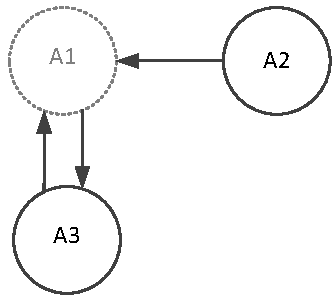
\includegraphics[scale=0.6]{img/Fig1}
\caption{Argumentation framework}
\label{fig:pras:example}
\end{figure}

Given an argumentation framework, the acceptability of arguments can be determined according to the appropriate argumentation semantics. The intuition is that an argument is acceptable if it is \emph{undefeated}, that is, any argument that attacks it, is itself defeated. Take, for example, the argumentation framework in Figure~\ref{fig:pras:example}. Argument A2 is undefeated because it has no attackers. This makes A1 defeated, because one of its attackers, A2, is undefeated. A3 is then also undefeated, since its only attacker, A1, is defeated by A2. Thus, the set of undefeated (justified) arguments given the argumentation framework in Figure~\ref{fig:pras:example} is $\{$A2, A3$\}$. 

In some cases, it is more difficult to determine whether or not an argument is defeated. Take, for example, the argumentation framework with just A1 and A3: they attack each other, they are alternatives and without any explicit preference, it is impossible to choose between the two. It is, however, possible to include explicit preferences between arguments when determining argument acceptability \cite{Amgoud}. Take, for example, A1 and A3. If we say that we prefer the goal ``XXX'' (A1) over the goal ``YYY'' (A3), we remove the attack from A3 to A1 (Figure~\ref{fig:pras:example2}, left). This makes A1 the only undefeated argument, whereas A3 is now defeated. It is also possible to give explicit arguments for preferences \cite{Modgil2009}. These arguments are then essentially attacks on attacks. For example, say we prefer A1 over A3 because ``XXX''. This can be rendered as a separate argument that attacks the attack from A3 to A1 (Figure~\ref{fig:pras:example2}, right), removing this attack and making $\{$A1, A4$\}$ the undefeated justified set of arguments.

\begin{figure}[ht]
\centering
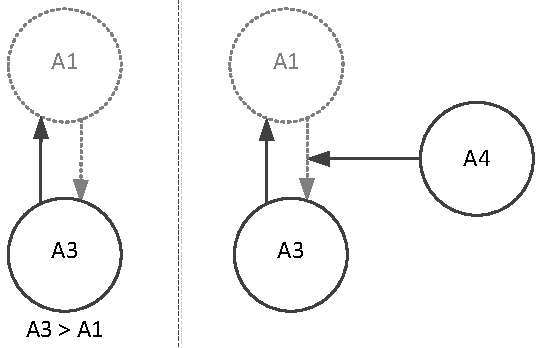
\includegraphics[scale=0.6]{img/Fig2}
\caption{Preferences between arguments}
\label{fig:pras:example2}
\end{figure}  

\subsubsection{Practical Reasoning and Goal Modeling}
\label{sect:background:pras:motivation}

Practical reasoning in the PRAS framework as described above provides a formally sound framework for defeasible reasoning about goals and actions that adheres to the acceptability semantics of Dung~\cite{Dung95} and its various extensions \cite{Amgoud, Modgil2009}. The usefulness of PRAS for the analysis of practical reasoning situations has been shown in different areas such as e-democracy~\cite{Atkinson2006}, law~\cite{???}, planning \cite{MedellinXXX} and choosing between safety critical actions \cite{}. The question in this paper is how PRAS can be adopted for use in goal modeling, so that we can capture the discussions between stakeholders that build a goal model as formal argumentation, thus adding a new evaluation technique for goal models that allows us to assess the \emph{acceptability} of elements of a goal model (as opposed to the \emph{satisfiability} \cite{}). 

PRAS  and GRL have some obvious similarities in that PRAS defines elements as actions, goals, values and GRL includes tasks, goals, softgoals. In previous work, we have already discussed how to translate practical reasoning arguments to GRL diagrams~\cite{}. For example, ... A similar approach, albeit without the explicit focus on practical reasoning, was taken by Jureta et al.~\cite{}, in which it translates similar structured arguments to goal diagrams. One of the problems of these approaches is that ...

The concept that appears in PRAS and not in GRL is \emph{circumstance}. In PRAS, an action $a$ is performed in current circumstances $R$, and by performing this action new circumstances $S$ are obtained. From this new circumstance $S$, another action may be performed again, and so on. In the AI literature, this type of reasoning usually referred to as ``AI planning''~\cite{weld1999recent}: from some initial state, find a sequence of actions such that a goal state is reached if these actions are executed. This planning approach is taken by a number of contributions using PRAS to create joint plans for a group of actors, often using a transition system as the underlying semantics~\cite{medellin2014}. However, in the early RE phase of an IS, one generally does not consider temporal planning. Decisions about the temporal order in which tasks should be executed are generally postponed until a later stage. In other words, goal modeling is not concerned with making plans, scenarios, or business processes for the information system. In URN (see section~\ref{sect:background:grl}) the distinction between goal modeling and business process modeling is clearly visible in the distinction between two separate modeling languages for the two activities. First, goal models are created in GRL and then, the use case maps (similar to business processes) are created in UCM. Therefore, when extending PRAS for GRL, we do not consider the notion of \emph{circumstances}.

The concept that appears in GRL but not in PRAS is \emph{resource}. A resource may be used by part of the system, or an actor, in order to perform a task or to reach a goal. Therefore, PRAS has to be extended with the notion of a resource in order for it to be applicable to GRL. %SGNew: to be applicable? don't understand the sentence. 

Finally, there are two concepts which appear in both models under different names. Where PRAS uses the notions ``action'' and ``value'', GRL uses the concepts ``task'' and respectively ``softgoal''. However, these two concepts are semantically identical.

With respect to relationships between concepts, the argument scheme PRAS from Section~\ref{sect:background:pras} contains the following relationships:\\

\noindent
R1. Actor $AG$ \emph{performs} action $A$\\
R2. Action $A$ \emph{realizes} goal $G$\\
R3. Goal $G$ \emph{promotes} value $S$\\
R4. Actor $AG$ \emph{has} goal $G$\\
R5. Actor $AG$ \emph{has} value $S$\\

\noindent

Relationships R4 and R5 are implicit in PRAS, but follow directly from its formulation (see~\cite{atkinson2007} for more details). The relationship ``promotes'' does not exist in GRL, but the relationship ``contributes to'' does, which is conceptually very similar. Therefore, we choose to use this relationship to formalize ``promotes'' relation.

As mentioned in Section~\ref{sect:background:grl}, GRL is a very non-restrictive modeling language, allowing intentional elements and links to be combined freely. Thus, GRL allows any links between any type of intentional element. PRAS, in contrast, only considers relationship R1-R5 above. As a result, the critical questions of PRAS are only applicable to a subset of all possible relationships in GRL. This, however, does not mean it is not possible to construct arguments and formulate critical questions for other relationship. In section~\ref{sect:implementation:implementation}, where we discuss the implementation of our tool, we explain in more detail that a user can straightforwardly add additional critical questions for other relationships as well.

\section{Argument Schemes for Goal Modeling (GMAS)}
\label{sect:gmas}

%SGNew: This pragprah seems redundant.  
%PRAS is not directly applicable to goal modeling in general, and GRL in particular. There are differences in the concepts used, and the relationships between these concepts. Some elements appear in PRAS that do not appear in GRL, some elements appear in GRL but not in PRAS, and some concepts appear in both formalisms but with different names. Moreover, GRL allows more relations between elements than the ones appearing in PRAS. 

%SGNew: What is the difference between PRAS and PAS? I think you should start this section with saying that based on what you defined in the last section, we developed a new argument schemes for goal modeling which is called GMAS. Then you can go ahead and talk that this is  the extension of PRAS, etc. I tried to reword.
%In this section, we first analyze these differences in more detail. A

In this section, we define our new argument schemes for GRL which is called Argument Schemes for Goal Modeling (GMAS) and its associated critical questions. GMAS is an extension of PRAS. PRAS  contains a single argument scheme PAS while GMAS  consists of nine argument schemes, which each can be used to instantiate an argument for particular part of a goal model. Each argument scheme is associated with critical questions that can be used to attack arguments or provide alternatives. This enables focused discussions about intentional elements and their relationships in a goal model. In the last subsection we illustrate applications of the argument schemes and critical questions with a simple example.

%After this, we introduce and motivate Argument Schemes for Goal Modeling (GMAS) and associated critical questions, which are an extension to PRAS. While PRAS contains a single argument scheme PAS, GMAS instead consists of nine argument schemes, which each can be used to instantiate an argument for particular part of a goal model. With each argument scheme we associate critical questions that can be used to attack arguments or provide alternatives. This enables focused discussions about elements and relationships of a goal model. In the last subsection we illustrate applications of the argument schemes and critical questions with a simple example.

\begin{table*}[h]
\centering
\begin{tabular}{|l|l|l|l|l|l|}
\hline
\multicolumn{2}{|c|}{\textbf{Argument scheme}} & \multicolumn{2}{c|}{\textbf{Critical Questions}} & \textbf{Attacks?}\\
\hline
AS1 & Actor $a$ has resource $R$ & CQ1 &Is the resource available? & Yes\\ %SGNew: tasks may also require resources to be available.. how do you show that?
\hline
AS2 & Actor $a$ can perform task $T$ & CQ2 &Is the task possible? & Yes\\
\hline
AS3 & Actor $a$ has goal $G$ & CQ3 & Can the desired goal be realized? & Yes\\
\hline
AS4 & Actor $a$ has softgoal $S$ & CQ4 & Is the softgoal a legitimate softgoal? & Yes\\
\hline
\hline
AS5 & Task $T$ realizes goal $G$ & CQ5a & Will the task realize the desired goal? & Yes\\
& & CQ5b & Are there alternative ways of realizing the same goal? \floris{How do you handle OR and XOR decompositions?} & No\\ %SGNew:What about decomposition of goals into goals?
\hline
AS6 & Task $T$ contributes to softgoal $S$ & CQ6a & Are there alternative ways of contributing to the same softgoal? & No\\
&& CQ6b & Does the task have a side effect which contribute negatively to the softgoal?&Yes\\
&& CQ6c & Does the task have a side effect which contribute negatively to some other softgoal? & No\\
&& CQ6d & Does the task contribute to some other softgoal?&No\\
&& CQ6e & Does the task preclude some other task which would contribute to some other softgoal?&Yes\\
\hline
AS7 & Goal $G$ contributes to softgoal $S$ & CQ7a & Does the goal contribute to the softgoal? & Yes\\
&& CQ7b & Does the goal contribute to some other softgoal? & No\\ %SGNew: What about contribution of goals to goals or softgoals to softgoals?
\hline
AS8 & Resource $R$ contributes to task $T$ & CQ8a & Is the resource required in order to perform the task? & Yes\\
&&CQ8b & Can other resources be used to perform the same task? & No\\
&&CQ8c & Is the resource required in order to perform the task? & Yes\\
&&CQ8d & Does using the resource make other resources unavailable? & Yes\\ %SGNew: Tasks need resources.. that is why tasks depends on resources.. I can't understand the contribution link between them.. resource doesn't have impact on the task..it should be dependency link. 
\hline
AS9 & Actor $a$ depends on actor $b$ & CQ9 & Does the actor depend on any actors? & No\\
\hline
\end{tabular}
\caption{Argument schemes and critical questions for GRL elements (CQ1-CQ4) and relationships (CQ5-CQ16), as well as whether answering the critical question unfavorably results in an attack on the original argument (right column).}
\label{table:argument-schemes}
\end{table*}

\subsection{The Argument Schemes and Critical Questions}

PRAS consists of the single argument scheme PAS.  However, our approach is to split this single scheme into a family of argument schemes, such that each separate argument scheme can be applied to a specific part of a goal model. Similar to PRAS, someone who does not accept the presumptive argument may challenge it by applying critical questions. We have modified Atkinson et al.'s original 16 questions associated with the scheme \cite{atkinson2006argumentation} by removing the ones that question the elements which are not part of GRL (\emph{circumstances}), by adding questions for additional elements in GRL (\emph{resources}), and finally by renaming concepts and relationships (e.g., the \emph{promotes} relationship).

We developed a total of 9 argument schemes and 18 critical questions, which are shown in table~\ref{table:argument-schemes}. Argument schemes AS1-AS4 can be instantiated for individual GRL elements, and each have a single critical question. CQ2-CQ4 are critical questions by Atkinson rephrased using the GRL terminology, while CQ1 is added in order to question a resource element, which does not appear in PRAS. AS5-AS9 are argument schemes for various GRL relationships between elements. As we mentioned before%SGNew: where?, 
this list is not meant to be exhaustive, since GRL does not put restrictions on any of the relationships and  in theory any type of elements can be combined with any other type of elements, using any relationship. Here, we merely use the critical questions developed by Atkinson et al. %SGNew: merely = only? I thought you modified them?
 
Answering a critical question results in the creation of a new argument, which may or may not attack the original arguments, depending on which question is answered. For instance, answering CQ1 with ``no'' results in a new argument attacking the argument that actor $a$ has resource $R$ available. In contrary, answering CQ5b with ``yes'' does not result in an attack on the original argument, but creates a new argument stating that some other task realizes the goal as well. In general, answering a critical questions can have two effects: %SGNew: why unfavorably?
\begin{enumerate}
\item
Answering the critical question unfavorably results in a new argument attacking the original argument (\emph{attack}).
\item
Answering the critical question unfavorably results in a new argument not attacking the original argument, but representing an alternative (\emph{no attack}).
\end{enumerate}
The last column of table~\ref{table:argument-schemes} shows for each critical question whether it results in an attack on the original argument or not. 

\floris{you do not provide a formal definition of GMAS} %SGNew: Agreed. What is missing here is a big picture or as we can say a methodology. I think it is important to introduce the methodology earlier and show how everything fit together. Also, to show what are the elements of GMAS and how it can be connected to GRL. You said, you extended PRAS and that is GMAS but can you show the extension?

\subsection{Example: Airport Assistant}

We now provide a simple scenario of arguments created by instantiating AS1-AS9, and demonstrate how new arguments can be generated through critical questions, possibly attacking the original arguments.

Consider a system for assisting users at the airport. The assistant should be able to guide users through the airport, inform them about delays, and provide other information such as the location of the check-in register for each airline company. When constructing a goal model for this system, one stakeholders argues that the user interface of the assistant should by easy to use, and that this can be realized by using a Graphical User Interface (GUI). We can formalize this as an instantiation of AS6:\\

\noindent
\textbf{$A_1$.} \emph{Task ``Use GUI'' contributes to softgoal ``easy to use'' (AS6)}.\\

\noindent
This argument can be subjected to critical questions. In this case, there are five critical questions that can be used on AS6, namely CQ6a-CQ6e. Critical question CQ6a asks for alternative solutions to contribute to softgoal ``easy to use''. One of the stakeholders may reply by stating a natural language interface is easy to use as well.\\

\noindent
\textbf{$A_2$.} \emph{Task ``Use NL interface'' contributes to softgoal ``easy to use'' (CQ6a/AS6)}.\\

\noindent
Note that $A_2$ does not create an attack on $A_1$, since both are valid tasks to contribute to the softgoal. Instead, $A_2$ actually generates new elements that will appear in the goal model.  Now both $A_1$ and $A_2$ can be questioned. Suppose CQ6b is used by a stakeholder to argue that a side effect of using a natural language interface is that not all users may be able to understand it. When using a GUI, it may be easier to let the user change its language.\\

\noindent
\textbf{$A_3$.} \emph{Task ``Use NL interface'' contributes negatively to softgoal ``easy to use'' because choosing a language is difficult (CQ6b).}\\

Suppose another stakeholder uses critical question CQ6c to question $A_1$: she notes that implementing a GUI is probably quite expensive, because they don't have a graphical designer, so they will have to outsource this.\\

\noindent
\textbf{$A_4$.} \emph{Task ``Use GUI'' contributes negatively to softgoal ``low costs''}.\\

\noindent
The resulting argumentation framework of these four arguments is shown in figure~\ref{fig:example:airport:arguments}. As we can see, argument $A_1$ and $A_4$ are both not attacked by any argument. However, $A_2$ and $A_3$ are in direct conflict. Recall from sectin~\ref{sect:background:pras} that the stakeholders now have to decide about their preferences. Suppose the stakeholders decide that argument $A_3$ is stronger, or more preferred, than $A_2$. As a result, the accepted arguments are $A_1, A_3$, and $A_4$. 

\begin{figure}
\centering
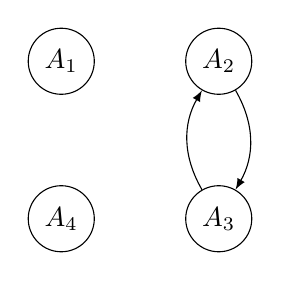
\begin{tikzpicture}[scale=2]
\node (a1) at (0,1) {$A_1$};
\node (a2) at (1,1) {$A_2$};
\node (a3) at (1,0) {$A_3$};
\node (a4) at (0,0) {$A_4$};
\draw [->] (a2) to [out=-60, in=60] (a3);
\draw [->] (a3) to [out=120, in=-120] (a2);
\end{tikzpicture}
\caption{Argumentation framework for Airport Assistant example.}
\label{fig:example:airport:arguments}
\end{figure}

It is now possible to translate this argumentation framework into a GRL model, which is shown in figure~\ref{fig:example:airport:grl}. Argument $A_1$ results in a contribution link from task ``use GUI'' to softgoal ``lower costs'', similarly for $A_4$. Since the conflict between $A_2$ and $A_3$ has been resolved in favor of $A_3$, there is a negative contribution link from task ``use NL interface'' to softgoal ``Easy to use''.

We can make a number of observations about the obtained GRL model and the underlying arguments:
\begin{itemize}
\item The underlying arguments contain information that is not represented in the GRL model. For instance, the decision to reject $A_2$ (i.e., that a natural language interface is easy to use) is not visible in the GRL model, but it is in the underlying arguments.
\item There is a direct relation between the accepted arguments and the elements that appear in the goal model. If an element or relation has an underlying accepted argument, it appears in the goal model, while rejected ones do not appear. Therefore, if the underlying arguments change \--- for instance if the stakeholders change their preference from $A_2$ to $A_3$ \-- then the resulting goal model changes as well.
\item In the current example, each GRL element and relation is supported by an argument. However, this is not required. One could imagine that the stakeholders choose to add additional elements to the goal model without rationalizing them by arguments. We explain this in more detail in the RationalGRL methodology in section~\ref{sect:methodology}. 
\item Although it may be intuitively understandable how to translate argument $A_1-A_4$ and the argumentation framework of figure~\ref{fig:example:airport:arguments} into the GRL model of figure~\ref{fig:example:airport:grl}, we have not yet formally specified how to make the translation from GMAS to GRL, and visa versa.
\end{itemize}

In this section, we have fulfilled requirement three of the introduction: (3) it (the practical reasoning and argumentation theory) must be adaptable for use in goal modeling. However, we have not yet considered the fourth requirement: (4) the adapted theory must produce repeatable results that can be formalized and implemented. This is what we do in the next section by providing formal mappings from GMAS to GRL, and discussing implementation details.

\begin{figure}
\centering
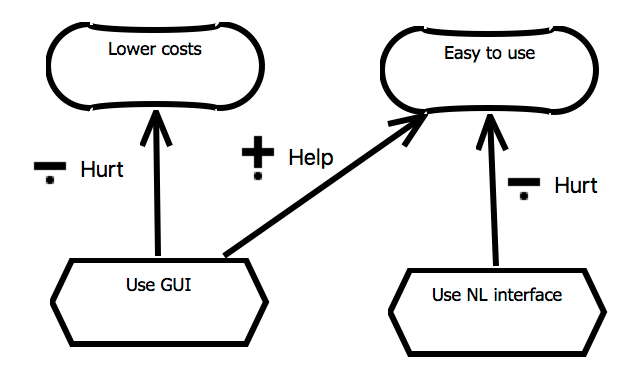
\includegraphics[scale=0.35]{img/grl_example_airport}
\caption{GRL model for Airport Assistant example.}
\label{fig:example:airport:grl}
\end{figure}

\section{Mapping GMAS to GRL: Metamodel and Implementation}
\label{sect:implementation}

\begin{figure*}[h]
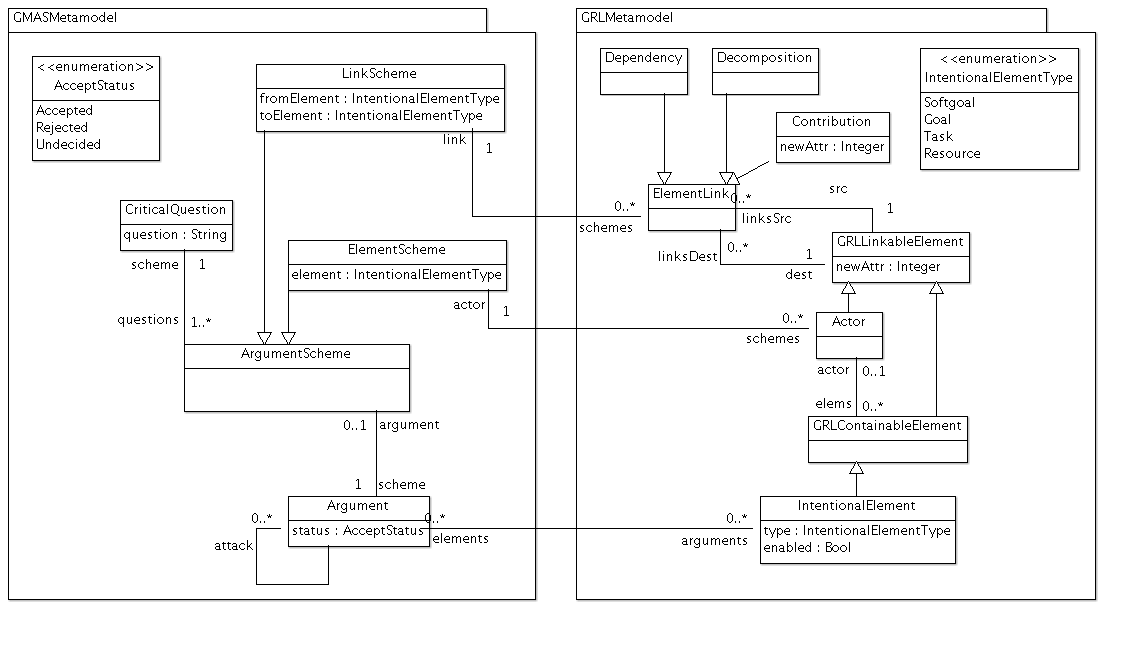
\includegraphics[scale=0.45]{img/ClassDiagram}
\caption{Metamodel specification of GMAS and GRL}
\label{fig:metamodel}
\end{figure*}
\floris{we have no formal definition of GMAS, so proposing a formal mapping will be difficult}
In the previous section, we adapted and extended the practical reasoning framework PRAS for use in goal modeling and developed  nine Argument Schemes for Goal Modeling (GMAS). These argument schemes can be instantiated to create arguments for elements and relationships in a GRL model. We introduced critical questions that can be used to construct counter arguments or alternatives, and we provided an example in which we obtained a GRL model from a GMAS specification. However, we did not yet create a formal language for GMAS, nor did we map it to GRL. This is what we do in the current section. We provide a formal specification of GMAS in terms of a metamodel, and we link it with the GRL metamodel. Using this mapping, we detail how to translate an argumentation framework into a GRL model and vice versa. The metamodel is the starting point for the tool we developed as an extension of jUCMNav. We present this tool in the last subsection, together with the visual language we developed for our extension.

\subsection{GMAS Metamodel Specification}
\label{sect:implementation:metamodel}

The UML metamodel of GMAS is shown on the left hand side of figure~\ref{fig:metamodel}.


\subsection{Mappings between GMAS and GRL}
\label{sect:implementation:mappings}

\subsubsection{Information Mappings}

\subsubsection{Formal Mappings}

\subsection{Implementation into jUCMNAv}
\label{sect:implementation:implementation}

\section{The RationalGRL Methodology}
\label{sect:methodology}

The methodology we propose in this paper is visualized in figure~\ref{fig:rationalgrl-methodology}. There are two main activities, depicted in grey, namely "goal modeling" and "argumentation". These are two separate activities that are being done in parallel. 

\begin{figure}[ht]
\centering

\includegraphics[scale=0.4]{img/methodology}
\caption{The RationalGRL Methodology}
\label{fig:rationalgrl-methodology}
\end{figure}

\section{Empirical Evaluation}
\label{sect:evaluation}

\section{Related Work}
\label{sect:relatedwork}

There are several contributions that relate argumentation-based techniques with goal modeling. The contribution most closely related to ours is the work by Jureta \emph{et al.}~\cite{Jureta:RE2008}. This work proposes ``Goal Argumentation Method (GAM)'' to guide argumentation and justification of modeling choices during the construction of goal models. One of the elements of GAM is the translation of formal argument models to goal models (similar to ours). In this sense, our \textsf{RationalGRL} framework can be seen as an instantiation and implementation of  part of the GAM. One of the main contribution of \textsf{RationalGRL} is that it also takes the acceptability of arguments as determined by the argumentation semantics \cite{Dung1995} into account when translating from arguments to goal models.  \textsf{RationalGRL} also provides tool support for argumentation, i.e. Argument Web toolset, to which OVA belongs \cite{bex2013implementing}, and for goal modeling, i.e. jUCMNav~\cite{jUCMNav}. Finally, \textsf{RationalGRL} is based on the practical reasoning approach of \cite{Atkinson2014}, which itself is also a specialization of Dung's~\cite{Dung1995} abstract approach to argumentation. Thus, the specific critical questions and counterarguments based on these critical question proposed by~\cite{Atkinson2014} can easily be incorporated into \textsf{RationalGRL}. 

\textsf{RationalGRL} framework is also closely related to frameworks that aim to provide a design rationale (DR)~\cite{shum2006hypermedia}, an explicit documentation of the reasons behind decisions made when designing a system or artefact. DR looks at issues, options and arguments for and against the various options in the design of, for example, a software system, and provides direct tool support for building and analyzing DR graphs. One of the main improvements of \textsf{RationalGRL} over DR approaches is that \textsf{RationalGRL} incorporates the formal semantics for both argument acceptability and goal satisfiability, which allow for a partly automated evaluation of goals and the rationales for these goals. 

Arguments and requirements engineering approaches have been combined by, among others, Haley \emph{et al.}~\cite{haley2005arguing}, who use structured arguments to capture and validate the rationales for security requirements. However, they do not use goal models, and thus, there is no explicit trace from arguments to goals and tasks. Furthermore, like~\cite{Jureta:RE2008}, the argumentative part of their work does not include formal semantics for determining the acceptability of arguments, and the proposed frameworks are not actually implemented. Murukannaiah \emph{et al.}~\cite{murukannaiah2015resolving} propose Arg-ACH, an approach to capture inconsistencies between stakeholders' beliefs and goals, and resolve goal conflicts using argumentation techniques.

\section{Conclusions and Future Work}
\label{sect:conclusion}

In this paper, we developed and implemented a framework to trace back elements of GRL models to arguments and evidence that derived from the discussions between stakeholders. We created a mapping algorithm from a formal argumentation theory to a goal model, which allows us to compute the evaluation values of the GRL IEs based on the formal semantics of the argumentation theory. 

There are many directions of future work. There are a large number of different semantics for formal argumentation, that lead to different arguments being acceptable or not. It would be very interesting to explore the effect of these semantics on goal models. Jureta \emph{et al.} develop a methodology for clarification to address issues such as ambiguity, overgenerality, synonymy, and vagueness in arguments. Atkinson \emph{et al.}~\cite{atkinson2007} define a formal set of critical questions that point to typical ways in which a practical argument can be criticized. We believe that critical questions are the right way to implement Jureta's methodology, and our framework would benefit from it. In addition, currently, we have not considered the \emph{Update} step of our framework (Figure~\ref{fig:overview}). That is, the translation from goal models to argument diagrams is still missing. The \emph{Update} step helps analysts change parts of the goal model and analyze its impact  on the underlying argument diagram. Finally, the implementation is currently a browser-based mapping from an existing argument diagramming tool to an existing goal modeling tool. By adding an argumentation component to jUCMNav, the development of goal models can be improved significantly. 

\section*{Acknowledgments}
Marc van Zee and Diana Marosin are funded by the National Research Fund (FNR), Luxembourg, by the  RationalArchitecture project.

\bibliographystyle{abbrv}
\bibliography{references}

\end{document}